% !TEX TS-program = xelatex
% !BIB TS-program = bibtex
\documentclass[12pt,letterpaper]{article}
\usepackage{style/dsc180reportstyle}

\title{Training-based versus training-free \\ differential privacy for data synthesis}

\author{Mehak Kapur \\
  {\tt mekapur@ucsd.edu} \\\And
  Hana Tjendrawasi  \\
  {\tt htjendrawasi@ucsd.edu} \\\And
  Jason Tran \\
  {\tt jat037@ucsd.edu} \\\And
  Phuc Tran \\
  {\tt pct001@ucsd.edu} \\\And
  Yu-Xiang Wang \\
  {\tt yuxiangw@ucsd.edu} \\}

\begin{document}
\maketitle

\begin{abstract}
Differentially private synthetic data generation enables the release of realistic datasets while protecting individual privacy. Two paradigms dominate current research: training-based methods such as differentially private stochastic gradient descent (DP-SGD), which inject noise during model optimization, and training-free methods such as Private Evolution (PE), which achieve privacy through inference-only access to foundation models. We investigate both approaches on Intel's Driver and Client Applications (DCA) telemetry corpus, a multi-table dataset comprising system metadata, power and thermal instrumentation, application usage, and browsing behavior across one million Windows clients. Our evaluation centers on a benchmark of 21 analytical SQL queries spanning aggregate statistics, ranked lists, geographic breakdowns, histograms, and complex pivots. For the training-based approach, we construct a unified wide table (one row per client, 307 encoded features) and train a differentially private variational autoencoder under $\varepsilon = 4.0$ at $\delta = 10^{-5}$. The model preserves categorical joint distributions: 42 of 50 countries present in the synthetic data receive the correct most-popular browser in a ranking query. All continuous metrics fail with relative errors exceeding 99\%, a consequence of extreme zero-inflation in the wide table, where 93--99.9\% of numeric columns are structurally zero. This sparsity failure identifies a fundamental limitation of wide-table approaches to multi-table DP synthesis. Experiments with Private Evolution under matched privacy budgets are planned to assess whether training-free methods better handle sparse, heterogeneous telemetry data.
\end{abstract}

\begin{center}
Code: \url{https://github.com/jktrns/DSC180B-Q2}
\end{center}

\maketoc
\clearpage

\section{Introduction}

\subsection{Motivation}

Organizations routinely collect detailed telemetry from their products to drive business decisions. Engineers use it to diagnose failures, product teams analyze usage trends, and analysts extract insights that shape product roadmaps. The same granularity that makes telemetry valuable also makes it sensitive. Browsing patterns, work schedules, and device fingerprints can re-identify specific individuals even after conventional anonymization.

Privacy regulations such as GDPR and CCPA, along with institutional policies, increasingly restrict how such data can be stored, shared, and analyzed. The resulting tension between data utility and privacy protection motivates the development of \textit{synthetic data generation}: producing artificial datasets that preserve the statistical properties necessary for analysis while providing formal guarantees that no individual's information can be recovered.

Two paradigms have emerged for generating synthetic data with rigorous privacy guarantees. \textit{Training-based methods} optimize generative models under constraints that bound individual influence, adding calibrated noise during the training process. \textit{Training-free methods} leverage pre-trained foundation models through black-box API access, achieving privacy through carefully designed selection mechanisms rather than private optimization. Both approaches have demonstrated success in isolation on image and text benchmarks, yet no comprehensive comparison exists under controlled experimental conditions with realistic analytical workloads on multi-table relational data.

This project provides that comparison. We implement both paradigms on Intel's Driver and Client Applications (DCA) telemetry corpus and evaluate them against a benchmark of 21 SQL queries representative of production analytics, measuring which approach better preserves query fidelity under equivalent privacy budgets.

\subsection{Prior work}

Differential privacy, introduced by \citet{dwork2014algorithmic}, provides the foundational framework for our privacy guarantees. A randomized mechanism $\mathcal{M}$ is $(\varepsilon, \delta)$-differentially private if for all neighboring databases $D, D'$ differing by one record and all measurable output sets $S$:
\begin{equation}
    \Pr[\mathcal{M}(D) \in S] \leq e^{\varepsilon} \Pr[\mathcal{M}(D') \in S] + \delta.
\end{equation}
The parameter $\varepsilon$ controls the privacy-utility tradeoff: smaller values confer stronger privacy at the cost of noisier outputs. The slack $\delta$ permits rare violations and must remain negligible relative to the database size. The work established key mechanisms (Laplace, Gaussian, exponential) for releasing numeric queries, along with composition theorems demonstrating that privacy loss accumulates across multiple analyses.

\citet{abadi2016deep} extended differential privacy to deep learning through DP-SGD. Standard gradient descent leaks information through the unbounded influence any single training example can exert on model parameters. DP-SGD bounds this influence by clipping each per-sample gradient to a fixed $\ell_2$ norm and injecting calibrated Gaussian noise to mask individual contributions. The accompanying \textit{moments accountant} yields substantially tighter privacy bounds than naive composition, enabling practical deep learning under modest privacy budgets.

\citet{ghalebikesabi2023differentially} demonstrated that fine-tuning diffusion models with DP-SGD generates synthetic images of reasonable quality, though their approach requires substantial privacy budgets ($\varepsilon \approx 32$ for CIFAR-10). This motivates the search for methods that achieve comparable fidelity at lower $\varepsilon$.

\citet{lin2025differentiallyprivatesyntheticdata} introduced Private Evolution (PE), a fundamentally different paradigm that avoids model training entirely. PE operates through black-box API access to pre-trained foundation models, iteratively evolving synthetic samples by computing differentially private nearest-neighbor histograms. Each private data point votes for its nearest synthetic candidate; Gaussian noise is added to the vote histogram, and candidates are resampled according to the noisy distribution. PE achieved FID $\leq 7.9$ at $\varepsilon = 0.67$ on CIFAR-10, a substantial improvement over DP-Diffusion in both privacy cost and output quality. The privacy analysis is simple: each iteration releases one Gaussian mechanism, and $T$ iterations compose to a single mechanism with noise multiplier $\sigma / \sqrt{T}$.

\citet{xie2024differentiallyprivatesyntheticdata} extended PE to text through Aug-PE, introducing fill-in-the-blanks variation, adaptive text lengths, and rank-based selection. Aug-PE with GPT-3.5 outperformed DP-finetuning baselines at the same privacy budget while running 12--66$\times$ faster.

\citet{swanberg2025apiaccessllmsuseful} adapted PE for tabular data using a workload-aware distance function that measures proximity in terms of query-relevant predicates rather than raw feature similarity. Their central finding is negative: API access to large language models does not yet improve differentially private tabular synthesis beyond established marginal-based baselines such as MST and JAM. This result informs our expectations for applying PE to the DCA telemetry corpus.

\newpage

\section{Data and problem statement}

\subsection{Intel DCA telemetry data}

Our investigation uses the Intel Driver and Client Applications (DCA) telemetry dataset, a large-scale collection of system-level signals from Windows client machines. The corpus comprises approximately 30 interrelated tables organized around a globally unique identifier (\texttt{guid}) assigned to each client system. We construct 19 reporting tables from the raw telemetry data, each aggregated to the \texttt{guid} level. The schema spans several categories:

\begin{itemize}
    \item \textit{Client metadata:} The \texttt{system\_sysinfo\_unique\_normalized} table (1{,}000{,}000 rows) provides static attributes including chassis type, country, OEM, RAM capacity, processor family, and a derived persona classification. This table serves as the anchor for all joins.

    \item \textit{Power and thermal:} Five tables capture physical instrumentation: processor power draw (\texttt{system\_hw\_pkg\_power}), total system power (\texttt{system\_psys\_rap\_watts}), processor temperature (\texttt{system\_pkg\_temp\_centigrade}), C0 state residency (\texttt{system\_pkg\_C0}), and clock frequency (\texttt{system\_pkg\_avg\_freq\_mhz}). Each provides per-\texttt{guid} weighted averages with sample counts.

    \item \textit{Battery and mobility:} The \texttt{system\_batt\_dc\_events} table summarizes battery utilization (duration on DC power, power cycle counts). Daily on/off/suspend durations are recorded in \texttt{system\_on\_off\_suspend\_time\_day}.

    \item \textit{Application behavior:} Foreground application usage by category (\texttt{system\_frgnd\_apps\_types}) and application wait times (\texttt{system\_userwait}).

    \item \textit{Web browsing:} The \texttt{system\_web\_cat\_pivot\_duration} table decomposes browsing across 28 categories (social, productivity, entertainment, gaming, etc.) by duration. A companion table (\texttt{system\_web\_cat\_usage}) provides per-browser aggregate statistics.

    \item \textit{Network and memory:} Network bytes sent and received (\texttt{system\_network\_consumption}) and RAM utilization statistics (\texttt{system\_memory\_utilization}).

    \item \textit{Display:} Connected display devices with connection type, resolution, and duration by AC/DC state (\texttt{system\_display\_devices}).
\end{itemize}

\subsection{Analytical query workload}

The practical utility of synthetic telemetry data is determined by its ability to support real analytical workloads. We operationalize this through a benchmark suite of 24 SQL queries developed by Intel analysts. Of these, 21 are feasible given our data coverage; 3 are permanently infeasible due to missing power consumption tables for which no viable raw source exists. The 21 feasible queries span five categories:

\begin{enumerate}
    \item \textit{Aggregate statistics with joins} (6 queries): weighted averages across multiple tables joined on \texttt{guid}, testing whether cross-table correlations survive synthesis.
    \item \textit{Ranked top-$k$} (7 queries): window functions producing ranked lists of applications, processes, or browsers, testing whether relative orderings are preserved.
    \item \textit{Geographic and demographic breakdowns} (4 queries): segmentation by country, processor generation, or persona, testing preservation of conditional distributions.
    \item \textit{Histograms and distributions} (2 queries): binned aggregations testing whether distributional shapes survive synthesis.
    \item \textit{Complex multi-way pivots} (2 queries): high-dimensional joint distributions across browsing categories, devices, or user segments.
\end{enumerate}

\subsection{Formal benchmark definition}

Let $\mathcal{Q} = \{q_1, \ldots, q_{21}\}$ denote our SQL query benchmark. Each query $q_j$ maps a database instance to a result set $q_j(D) \in \mathcal{R}_j$, where $\mathcal{R}_j$ may be a scalar, vector, or table. The query discrepancy for synthetic data $\tilde{D}$ is:
\begin{equation}
    \Delta_j(D, \tilde{D}) = d_j\bigl(q_j(D),\; q_j(\tilde{D})\bigr),
\end{equation}
where $d_j$ is a distance metric appropriate to the result type: relative error for scalars, Spearman's $\rho$ for rankings, and total variation for histograms. The aggregate benchmark score is:
\begin{equation}
    \text{Score}(\tilde{D}) = \frac{1}{|\mathcal{Q}|} \sum_{j=1}^{|\mathcal{Q}|} \mathbf{1}\bigl[\Delta_j(D, \tilde{D}) \leq \tau_j\bigr],
\end{equation}
where $\tau_j$ is a query-specific tolerance threshold. A synthetic dataset passes the benchmark if it achieves a high score, indicating that analysts could substitute $\tilde{D}$ for $D$ without materially affecting conclusions.

\subsection{Research questions}

Given the 21-query benchmark and matched privacy budgets, we investigate:

\begin{enumerate}
    \item Under matched $(\varepsilon, \delta)$, which method achieves higher benchmark scores? Which query types exhibit the largest discrepancy?
    \item Does error compound across multi-table joins, or does the synthesis mechanism preserve joint distributions adequately?
    \item Which method better preserves minority class frequencies (prevalence $< 5\%$)?
    \item Do classifiers trained on synthetic data achieve comparable accuracy to those trained on real data?
    \item What are the wall-clock time and resource requirements for each method?
\end{enumerate}

\newpage

\section{Methods}

\subsection{Wide-table construction}

The unit of synthesis is the \texttt{guid}. Each \texttt{guid} represents one client system, and the privacy guarantee is per-\texttt{guid}: neighboring databases differ by adding or removing all rows associated with a single device.

Synthesizing each reporting table independently would destroy cross-table correlations. Most benchmark queries join multiple tables on \texttt{guid}; if synthetic tables share no relationship, joins produce either zero matches (mismatched \texttt{guid}s) or random associations (correct \texttt{guid}s but uncorrelated attributes). Queries measuring cross-table relationships (e.g., ``average network consumption by chassis type'') would return meaningless results.

We therefore construct a single wide table with one row per \texttt{guid} containing all attributes and pre-aggregated metrics from every reporting table. For each reporting table, we compute \texttt{guid}-level aggregations of the columns referenced by benchmark queries. Multi-row-per-\texttt{guid} tables (e.g., web browsing by category) are pivoted into separate columns per category. All aggregations are LEFT JOINed onto the sysinfo anchor table (1{,}000{,}000 \texttt{guid}s).

The resulting wide table has 1{,}000{,}000 rows and 70 columns: 9 categorical attributes and 59 numeric metrics, plus \texttt{guid}. We encode categoricals via top-$k$ binning ($k = 50$, with remaining values grouped into ``Other'') and one-hot encoding. Numeric columns are clipped at the 99.9th percentile, transformed via $\log(1 + x)$ to reduce skew, and standardized with zero mean and unit variance. The final feature matrix has $1{,}000{,}000 \times 307$ entries (248 one-hot indicators plus 59 scaled numerics).

\subsection{DP-VAE architecture}

We train a differentially private variational autoencoder (DP-VAE) on the wide table. Let $x \in \mathbb{R}^{307}$ denote a \texttt{guid}-level feature vector. The encoder maps $x$ through two hidden layers of 512 units each to produce a 64-dimensional mean $\mu$ and log-variance $\log \sigma^2$. We sample $z = \mu + \sigma \odot \epsilon$ where $\epsilon \sim \mathcal{N}(0, I)$.

The decoder uses separate heads for categorical and numeric attributes:
\begin{itemize}
    \item 9 categorical heads, each producing logits over the corresponding column's vocabulary. Loss: cross-entropy.
    \item 1 numeric head mapping $z$ to 59 outputs. Loss: mean squared error.
\end{itemize}

The total loss is:
\begin{equation}
    \mathcal{L} = \sum_{c=1}^{9} \text{CE}(x_c, \hat{x}_c) + \text{MSE}(x_{\text{num}}, \hat{x}_{\text{num}}) + \text{KL}\bigl(q_\phi(z \mid x) \;\|\; \mathcal{N}(0, I)\bigr).
\end{equation}

The model has 505{,}971 trainable parameters.

\begin{algorithm}[h]
\caption{DP-VAE training with DP-SGD}
\label{alg:dpvae}
\SetKwInOut{KwInput}{Input}
\SetKwInOut{KwOutput}{Output}
\KwInput{Wide table $X \in \mathbb{R}^{n \times 307}$, target $\varepsilon^\star$, $\delta$, clip norm $C$, epochs $E$, batch size $B$}
\KwOutput{Trained parameters $\theta$, final $\varepsilon$}
Wrap optimizer with Opacus: $\sigma \gets \texttt{make\_private\_with\_epsilon}(\varepsilon^\star, \delta, E, B)$\;
\For{epoch $= 1, \ldots, E$}{
    \For{each batch $\{x_i\}_{i=1}^B \subset X$}{
        Encode: $(\mu_i, \log \sigma_i^2) \gets \text{Encoder}(x_i)$\;
        Sample: $z_i \gets \mu_i + \sigma_i \odot \epsilon_i$, \quad $\epsilon_i \sim \mathcal{N}(0, I)$\;
        Decode: $\hat{x}_i \gets \text{Decoder}(z_i)$\;
        Compute $\mathcal{L}_i = \text{CE}_i + \text{MSE}_i + \text{KL}_i$\;
        Clip: $\bar{g}_i \gets \nabla_\theta \mathcal{L}_i \cdot \min(1, C / \|\nabla_\theta \mathcal{L}_i\|_2)$\;
        Noise: $\tilde{g} \gets \frac{1}{B}\bigl(\sum_i \bar{g}_i + \mathcal{N}(0, \sigma^2 C^2 I)\bigr)$\;
        Update: $\theta \gets \theta - \eta \tilde{g}$\;
    }
}
$\varepsilon \gets \texttt{PrivacyAccountant.get\_epsilon}(\delta)$\;
\end{algorithm}

\subsection{DP-SGD training and privacy accounting}

We use the Opacus library to apply DP-SGD. Rather than manually selecting a noise multiplier, we use Opacus's \texttt{make\_private\_with\_epsilon} to automatically calibrate $\sigma$ for a target budget of $\varepsilon = 4.0$ at $\delta = 10^{-5}$. Privacy loss is tracked via the R\'{e}nyi differential privacy (RDP) accountant, which yields tighter bounds than basic composition.

Table~\ref{tab:hyperparams} reports the training configuration. The final privacy expenditure is $\varepsilon = 3.996$.

\begin{table}[h]
\centering
\begin{tabular}{lc}
\toprule
\textbf{Hyperparameter} & \textbf{Value} \\
\midrule
Encoder architecture & $307 \to 512 \to 512 \to (64\mu, 64\log\sigma^2)$ \\
Decoder architecture & $64 \to 512 \to 512 \to$ 9 categorical + 1 numeric head \\
Total parameters & 505{,}971 \\
Batch size & 4{,}096 \\
Epochs & 20 \\
Learning rate & $10^{-3}$ (Adam) \\
Max gradient norm $C$ & 1.0 \\
Noise multiplier $\sigma$ & auto-calibrated by Opacus \\
Target $\varepsilon$ & 4.0 \\
$\delta$ & $10^{-5}$ \\
Final $\varepsilon$ & 3.996 \\
Training time & 359.7 min (CPU) \\
\bottomrule
\end{tabular}
\caption{DP-VAE training configuration.}
\label{tab:hyperparams}
\end{table}

\subsection{Synthetic data generation and decomposition}

After training, we generate 1{,}000{,}000 synthetic \texttt{guid} records:

\begin{enumerate}
    \item Sample $z \sim \mathcal{N}(0, I_{64})$.
    \item Decode to produce categorical logits and numeric outputs.
    \item For each categorical column, sample from the softmax distribution over the vocabulary.
    \item For each numeric column, apply the inverse transformations: de-standardize, apply $\text{expm1}(x) = e^x - 1$, and clip to the observed range.
\end{enumerate}

The synthetic wide table is then decomposed back into 12 reporting table schemas by selecting the relevant columns for each table and assigning synthetic \texttt{guid}s. The original benchmark SQL queries execute unchanged on these synthetic reporting tables.

We evaluate 8 of the 21 feasible queries whose reporting tables are fully reconstructable from the wide-table columns. The remaining 13 queries require per-row columns not present in the wide table (e.g., per-process breakdowns for userwait, per-application data for foreground apps, per-display data for display devices).

\subsection{Private Evolution (planned)}

We plan to implement Private Evolution adapted for tabular data, following the framework of \citet{lin2025differentiallyprivatesyntheticdata} with the workload-aware distance function proposed by \citet{swanberg2025apiaccessllmsuseful}. The algorithm iteratively evolves a population of synthetic records through three steps per iteration:

\begin{enumerate}
    \item \textit{Candidate generation:} prompt a foundation model to produce variations of current synthetic records that conform to the DCA schema.
    \item \textit{Private selection:} compute a nearest-neighbor histogram in which each real record votes for its closest synthetic candidate under the workload-aware distance. Add Gaussian noise calibrated to the histogram sensitivity (1, since each \texttt{guid} contributes exactly one vote).
    \item \textit{Resampling:} resample the synthetic population according to the noisy histogram, retaining candidates that best approximate the real data distribution.
\end{enumerate}

Privacy follows from composition of $T$ Gaussian mechanisms, equivalent to a single mechanism with noise multiplier $\sigma / \sqrt{T}$. We will match the DP-SGD budget ($\varepsilon = 4.0$, $\delta = 10^{-5}$) for a controlled comparison.

Given \citeauthor{swanberg2025apiaccessllmsuseful}'s negative result on tabular PE (API access did not improve over marginal-based baselines), we treat this comparison as an empirical test of whether PE's advantages in the image and text domains transfer to heterogeneous, sparse telemetry data.

\newpage

\section{Results}

We evaluate the DP-VAE synthetic data on 8 of 21 feasible benchmark queries. The remaining 13 queries require per-row reporting table columns (e.g., per-process wait times, per-application focal durations) that are not present in the wide-table representation.

\subsection{Browser ranking preservation}

The \texttt{most\_popular\_browser\_in\_each\_country} query identifies the dominant browser in each country by system count. The real data produces rankings for 51 countries; the synthetic data covers 50 (the United Arab Emirates is absent). Of the 50 shared countries, the DP-VAE correctly identifies the most popular browser in 42 (84\% accuracy). Table~\ref{tab:browser-ranking} shows the 8 countries where the synthetic ranking diverges.

\begin{table}[h]
\centering
\begin{tabular}{lcc}
\toprule
\textbf{Country} & \textbf{Real} & \textbf{Synthetic} \\
\midrule
Australia & chrome & edge \\
Canada & chrome & edge \\
China & edge & chrome \\
Egypt & chrome & edge \\
Hong Kong & chrome & edge \\
Korea, Republic of & edge & chrome \\
United Kingdom & chrome & edge \\
United States & chrome & edge \\
\bottomrule
\end{tabular}
\caption{Countries where the DP-VAE assigns the wrong most-popular browser. All 8 mismatches involve a swap between chrome and edge, reflecting the global near-parity between these two browsers in prevalence.}
\label{tab:browser-ranking}
\end{table}

This result demonstrates that the DP-VAE preserves the joint distribution between \texttt{countryname\_normalized} and browser preference well enough to maintain rankings. The errors occur in countries where chrome and edge are close in prevalence, making the ranking sensitive to small perturbations.

\subsection{Browser usage percentages}

The \texttt{popular\_browsers} query computes the percentage of systems, instances, and total duration attributable to each of the three major browsers. Figure~\ref{fig:browser-usage} compares real and synthetic results.

\begin{figure}[h]
\centering
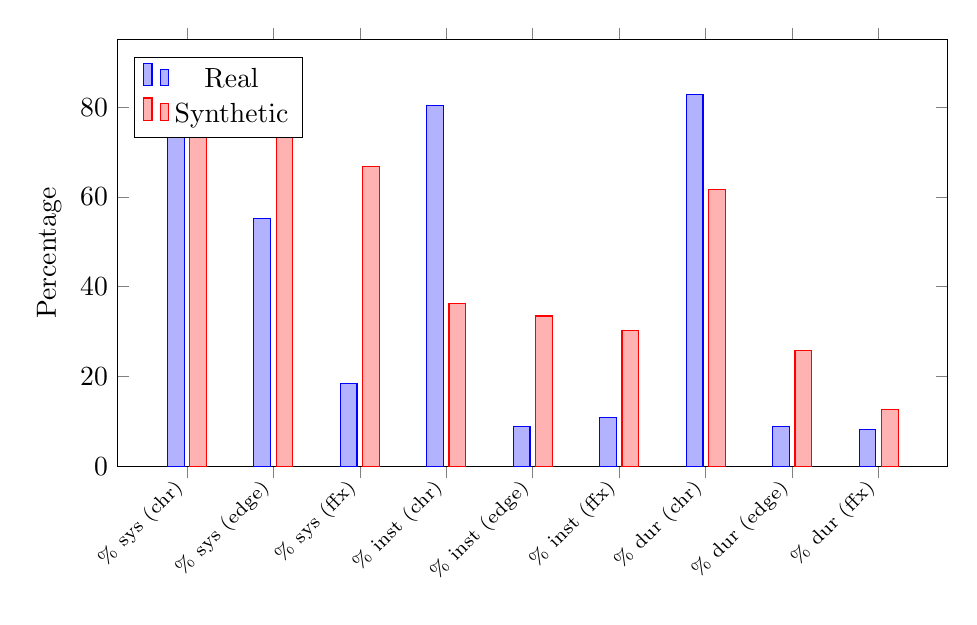
\begin{tikzpicture}
\begin{axis}[
    ybar,
    bar width=6pt,
    width=\linewidth,
    height=7cm,
    ylabel={Percentage},
    symbolic x coords={chrome-sys,edge-sys,firefox-sys,chrome-inst,edge-inst,firefox-inst,chrome-dur,edge-dur,firefox-dur},
    xtick=data,
    x tick label style={rotate=45, anchor=east, font=\scriptsize},
    legend style={at={(0.02,0.96)}, anchor=north west},
    ymin=0, ymax=95,
    xticklabels={\% sys (chr), \% sys (edge), \% sys (ffx), \% inst (chr), \% inst (edge), \% inst (ffx), \% dur (chr), \% dur (edge), \% dur (ffx)},
]
\addplot coordinates {
    (chrome-sys,82.05) (edge-sys,55.16) (firefox-sys,18.36)
    (chrome-inst,80.30) (edge-inst,8.91) (firefox-inst,10.79)
    (chrome-dur,82.89) (edge-dur,8.88) (firefox-dur,8.23)
};
\addplot coordinates {
    (chrome-sys,79.97) (edge-sys,73.90) (firefox-sys,66.78)
    (chrome-inst,36.24) (edge-inst,33.49) (firefox-inst,30.27)
    (chrome-dur,61.57) (edge-dur,25.73) (firefox-dur,12.70)
};
\legend{Real, Synthetic}
\end{axis}
\end{tikzpicture}
\caption{Browser usage metrics: percentage of systems, instances, and duration for chrome, edge, and firefox. The synthetic data preserves the relative ordering for duration but collapses the instance-level distribution toward uniformity ($\approx 33\%$ each), an artifact of the decomposition process assigning one row per \texttt{guid} per browser.}
\label{fig:browser-usage}
\end{figure}

The percent-systems metric is roughly preserved for chrome ($82.1\% \to 80.0\%$) but inflated for edge ($55.2\% \to 73.9\%$) and firefox ($18.4\% \to 66.8\%$). The percent-instances metric collapses to near-uniform ($\approx 33\%$ per browser) because the wide-table decomposition creates exactly one row per \texttt{guid} per browser, losing real instance-count variation.

\newpage

\subsection{Continuous metric failure}

All queries involving continuous metrics (power, temperature, frequency, network bytes, memory utilization, battery duration) produce synthetic values near zero, with relative errors exceeding 99\%. Table~\ref{tab:continuous-failure} reports representative values for the five-way chassis join query and other continuous queries.

\begin{table}[h]
\centering
\begin{tabular}{lccc}
\toprule
\textbf{Metric} & \textbf{Real} & \textbf{Synthetic} & \textbf{Rel.\ error} \\
\midrule
avg\_psys\_rap\_watts & 4.42 & 0.002 & $> 99\%$ \\
avg\_pkg\_c0 (\%) & 37.4 & 0.022 & $> 99\%$ \\
avg\_freq\_mhz & 1{,}582 & 0.009 & $> 99\%$ \\
avg\_temp\_centigrade & 44.5 & 0.003 & $> 99\%$ \\
avg\_bytes\_received & $7.4 \times 10^{16}$ & 1.12 & $> 99\%$ \\
avg\_percentage\_used (\%) & 42.6 & 0.0 & $100\%$ \\
avg\_duration (battery, min) & 144 & 0.11 & $> 99\%$ \\
\bottomrule
\end{tabular}
\caption{Real vs.\ synthetic values for continuous metrics (notebook chassis type where applicable). All synthetic values are near zero.}
\label{tab:continuous-failure}
\end{table}

Figure~\ref{fig:ram-utilization} illustrates the failure on the RAM utilization histogram. Real data shows a clear inverse relationship between RAM capacity and utilization percentage. The synthetic data reports 0\% utilization across all capacities.

\begin{figure}[h]
\centering
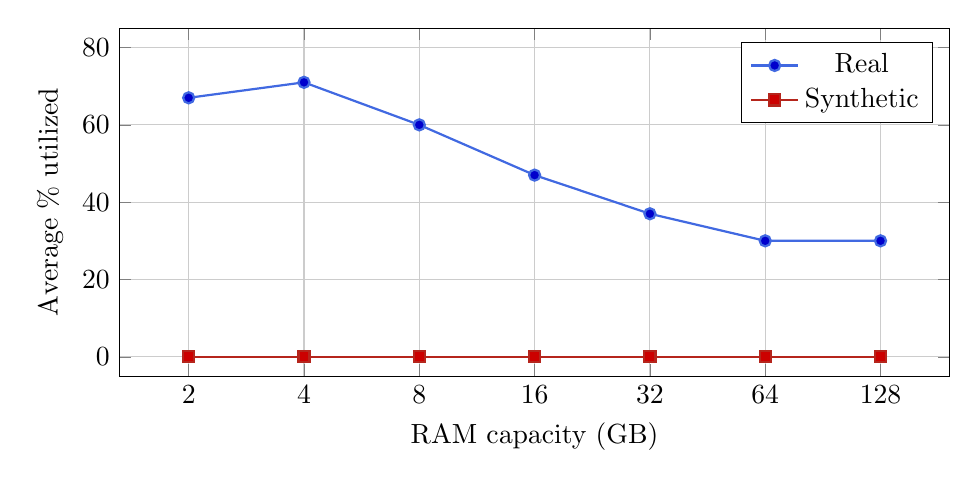
\begin{tikzpicture}
\begin{axis}[
    width=\linewidth,
    height=6cm,
    xlabel={RAM capacity (GB)},
    ylabel={Average \% utilized},
    xmode=log,
    log basis x=2,
    xtick={2,4,8,16,32,64,128},
    xticklabels={2,4,8,16,32,64,128},
    legend style={at={(0.98,0.96)}, anchor=north east},
    ymin=-5, ymax=85,
    grid=both,
    minor grid style={gray!20},
    major grid style={gray!40},
]
\addplot+[mark=*, thick, RoyalBlue] coordinates {
    (2,67) (4,71) (8,60) (16,47) (32,37) (64,30) (128,30)
};
\addlegendentry{Real}
\addplot+[mark=square*, thick, BrickRed] coordinates {
    (2,0) (4,0) (8,0) (16,0) (32,0) (64,0) (128,0)
};
\addlegendentry{Synthetic}
\end{axis}
\end{tikzpicture}
\caption{RAM utilization by capacity. Real data exhibits the expected inverse trend: devices with less RAM operate at higher utilization. The synthetic data produces 0\% utilization universally, as the memory columns in the wide table are zero for 93\% of \texttt{guid}s.}
\label{fig:ram-utilization}
\end{figure}

\subsection{Root cause: wide-table sparsity}

The continuous metric failure stems from extreme zero-inflation in the wide table. Most metric columns are nonzero for only a small fraction of the 1{,}000{,}000 \texttt{guid}s, because each event table covers a different subset of devices:

\begin{table}[h]
\centering
\begin{tabular}{lrr}
\toprule
\textbf{Metric source} & \textbf{Nonzero guids} & \textbf{Sparsity} \\
\midrule
PSYS RAP watts & 816 & 99.9\% \\
Average frequency & 613 & 99.9\% \\
Temperature & 622 & 99.9\% \\
C0 residency & 8{,}943 & 99.1\% \\
Network consumption & 37{,}224 & 96.3\% \\
Memory utilization & 69{,}552 & 93.0\% \\
\bottomrule
\end{tabular}
\caption{Nonzero coverage per metric in the wide table. The PSYS RAP, frequency, and temperature metrics have data for fewer than 0.1\% of \texttt{guid}s.}
\label{tab:sparsity}
\end{table}

The VAE optimizes mean squared error on these columns. When 93--99.9\% of values are zero, the loss-minimizing strategy is to generate near-zero values for all \texttt{guid}s. The KL divergence term further regularizes the latent space toward the standard normal, discouraging the model from learning a thin nonzero mode that accounts for less than 1\% of the data.

A secondary consequence is system count inflation. The five-way chassis join returns 104 real \texttt{guid}s (those with data in all five metric tables simultaneously). The synthetic data returns over 163{,}000 matches because the model generates small positive residuals for all \texttt{guid}s, causing the INNER JOIN to match far more rows than it should.

\newpage

\section{Discussion}

The DP-SGD results provide a direct answer to research question (2): error compounds dramatically across multi-table joins when the synthesis approach introduces structural sparsity artifacts. The wide-table design is correct in principle, as it preserves the joint distribution across tables by construction. In practice, it creates a feature matrix where most columns are nearly degenerate. The VAE collapses these sparse columns to their mode (zero), destroying any signal in the nonzero tail.

The browser ranking result demonstrates that the approach succeeds for well-populated categorical attributes. The joint distribution between country and browser preference is dense (every \texttt{guid} has a country; most have web browsing data), so the model learns a meaningful conditional distribution that preserves top-1 rankings in 84\% of countries.

Several mitigation strategies warrant investigation:

\begin{itemize}
    \item A two-stage model: first a Bernoulli model for zero vs.\ nonzero per column, then a conditional model for nonzero values only.
    \item Per-table independent synthesis (sacrificing cross-table correlations) as a baseline to isolate the sparsity effect.
    \item A zero-inflated loss function replacing plain MSE for numeric columns.
    \item Restricting the wide table to \texttt{guid}s with sufficient coverage (e.g., present in $\geq 3$ metric tables).
\end{itemize}

Private Evolution may be better suited to this setting. Rather than learning a generative model over the full 307-dimensional feature space, PE operates in an embedding space and uses a foundation model as a proposal mechanism. If the foundation model can generate plausible telemetry records with realistic sparsity patterns (i.e., most records have data in only a few metric tables), PE could preserve the heterogeneous coverage structure that the VAE collapses.

\section{Conclusion}

We presented a controlled evaluation of differentially private synthetic data generation on Intel's DCA telemetry corpus. The DP-VAE trained with DP-SGD ($\varepsilon = 3.996$, $\delta = 10^{-5}$) preserves categorical joint distributions (42/50 countries receive the correct top browser) but fails on all continuous metrics due to extreme zero-inflation in the wide-table representation.

This result identifies the sparsity structure of multi-table joins as a critical factor in the success or failure of DP synthetic data generation. When coverage varies across tables (as it does in any real multi-table dataset), a unified representation concentrates nearly all probability mass at zero for sparse columns, and standard generative models learn to reproduce this mode.

Our evaluation so far covers only the DP-SGD paradigm. The comparison with Private Evolution, using matched privacy budgets and the same 21-query benchmark, will determine whether training-free methods handle the heterogeneous structure of relational telemetry data more effectively.

\newpage

\makereference

\nocite{*}
\bibliography{reference}
\bibliographystyle{style/dsc180bibstyle}

\newpage
\appendix

\section{Project proposal}

The following is reproduced from the Q2 project proposal submitted in Fall 2025.

\subsection{Problem statement}

Organizations routinely collect detailed telemetry from their products that drive critical business decisions. The same granularity that makes telemetry valuable also makes it sensitive. Differential privacy (DP) provides a rigorous mathematical framework for releasing data while bounding the influence of any individual record. Two paradigms have emerged for generating differentially private synthetic data: training-based methods (DP-SGD) that inject noise during model optimization, and training-free methods (Private Evolution) that achieve privacy through black-box API access to foundation models.

We implement and compare both approaches on Intel's Driver and Client Applications (DCA) telemetry corpus, evaluating against a benchmark of analytical SQL queries representative of production business intelligence workloads. Under matched privacy budgets ($\varepsilon = 4.0$, $\delta = 10^{-5}$), we assess query fidelity, statistical preservation, and computational cost to determine whether training-free methods can match training-based approaches on real multi-table relational data.

\subsection{Data}

The DCA telemetry corpus comprises approximately 30 interrelated tables organized around a globally unique client identifier (\texttt{guid}). Tables span system metadata, power and thermal instrumentation, battery usage, application behavior, web browsing, network consumption, and display devices. We construct 19 reporting tables from the raw data, each aggregated to the \texttt{guid} level, and define a benchmark of 21 feasible SQL queries covering aggregate statistics with joins, ranked top-$k$ lists, geographic and demographic breakdowns, histograms, and complex multi-way pivots.

\subsection{Methods}

For training-based synthesis, we implement a differentially private variational autoencoder (DP-VAE) using PyTorch and the Opacus library, with privacy guarantees via DP-SGD (per-sample gradient clipping and calibrated noise injection). For training-free synthesis, we implement Private Evolution using black-box API access to foundation models, achieving privacy through differentially private nearest-neighbor histograms. Both methods are evaluated under matched privacy budgets on the 21-query SQL benchmark.

\subsection{Research questions}

\begin{enumerate}
    \item Under matched $(\varepsilon, \delta)$, which method achieves higher scores on the SQL query benchmark?
    \item Does error compound across multi-table joins?
    \item Which method better preserves minority class frequencies?
    \item Do classifiers trained on synthetic data achieve comparable accuracy to those trained on real data?
    \item What are the wall-clock time and resource requirements for each method?
\end{enumerate}

\subsection{Expected outputs}

\begin{enumerate}
    \item Technical report with implementation details, privacy analysis, and query-by-query benchmark results.
    \item SQL benchmark suite (21 queries with natural language specifications, SQL code, and evaluation scripts).
    \item Two differentially private synthetic DCA datasets (one DP-SGD, one PE) with documented privacy guarantees.
    \item Project website with visualizations and deployment guidelines.
    \item Open-source implementations for preprocessing, training, generation, and evaluation.
\end{enumerate}

\newpage

\section{Contributions}

\noindent Jason Tran: Designed and built the complete data infrastructure, including 19 reporting tables aggregated from raw DCA telemetry data, a 24-query SQL benchmark suite, and all 5 analysis notebooks. Implemented the wide-table synthesis methodology, trained the DP-VAE with DP-SGD using Opacus, conducted all benchmark evaluations, and wrote this report.

\medskip
\noindent Mehak Kapur:

\medskip
\noindent Hana Tjendrawasi:

\medskip
\noindent Phuc Tran:

\end{document}
